
\documentclass{article}

% Page layout and margins
\usepackage[
	a4paper,
	bindingoffset=0.2in,
	left=1in,
	right=1in,
	top=1in,
	bottom=1in,
	footskip=.25in
]{geometry}

% Language
\usepackage[brazil]{babel}

% Math and symbols
\usepackage{amsmath, amssymb, mathtools}

% Algorithms
\usepackage[linesnumbered,ruled,vlined]{algorithm2e}

\SetKwIF{If}{ElseIf}{Else}{if}{:}{else if}{else}{end}
\SetKwFor{For}{for}{:}{end}
\SetKwRepeat{Do}{do}{while}
\SetKwProg{Function}{def}{:}{}

% Graphics and figures
\usepackage{graphicx}
\usepackage{subcaption}
\usepackage{caption}
\usepackage{float}
\usepackage{adjustbox}
\usepackage{tikz}

% Text formatting and layout
\usepackage{indentfirst}
\usepackage{fancyhdr}
\usepackage{quoting}
\usepackage{xcolor} % no need for [dvipsnames] unless you need extended colors

% URLs and hyperlinks
\usepackage{hyperref}
\usepackage{url}

% Code listings (optional, if you actually use it)
\usepackage{listings}

% Framed boxes (optional, if you use them)
\usepackage{tcolorbox}
\usepackage{mdframed}

% Citations
\usepackage{amsrefs} % or biblatex if preferred
\usepackage{cite}

\usepackage{setspace} % Para definir espaçamento entre linhas. (\onehalfspacing, \singlespacing, \doublespacing)
\usepackage{enumitem} % Para customizar listas (itemize, enumerate, etc.)

\usepackage{wrapfig}

\definecolor{lightgray}{RGB}{240,240,240}

\newenvironment{blockquote}[1][lightgray]{\begin{mdframed}[
	leftline=true,
	topline=false,
	bottomline=false,
	rightline=false,
	linecolor=gray,
	linewidth=2pt,
	backgroundcolor=#1,
	skipabove=\baselineskip,
	skipbelow=\baselineskip,
	innerleftmargin=10pt,
	innerrightmargin=10pt,
	innertopmargin=5pt,
	innerbottommargin=5pt]
}
{\end{mdframed}}

% Counter for proof lines
\newcounter{proofline}

% Custom paired delimiters
\DeclarePairedDelimiter{\floor}{\lfloor}{\rfloor}
\DeclarePairedDelimiter{\ceil}{\lceil}{\rceil}
\DeclarePairedDelimiter{\abs}{\lvert}{\rvert}
\DeclarePairedDelimiter{\parens}{(}{)}
\DeclarePairedDelimiter{\curly}{\{}{\}}

% Box spacing tweaks
\setlength{\fboxsep}{0pt}
\setlength{\fboxrule}{1.4pt}

% Paragraph indent
\setlength{\parindent}{2em}

% Page style setup
\pagestyle{fancy}
\lhead{\footnotesize {\sc }}
\chead{}
\rhead{\footnotesize {\sc mac-ime-usp}}
\lfoot{}
\cfoot{}
\rfoot{\thepage}

\renewcommand{\headrulewidth}{0.5pt}
\renewcommand{\footrulewidth}{0.5pt}

\begin{document}

\begin{titlepage}

\begin{center}
	
	\begin{figure}[H]
		\centering
		
\includegraphics[width=0.3\textwidth]{logo-small.png} % Ajuste o caminho da imagem conforme necessário
	\end{figure}

	\vspace{2cm}

	{\Large \sc UNIVERSIDADE DE SÃO PAULO} \\
	{\Large \sc INSTITUTO DE MATEMÁTICA E ESTATÍSTICA} \\ [0.7cm]
	{\sc DEPARTAMENTO DE CIÊNCIA DA COMPUTAÇÃO} \\

	\vspace{2cm}

	\rule{\linewidth}{2pt}
	
	\vspace{0.2em} % Ajuste ao seu gosto
	{\Large \bfseries 
		O Problema da Visita de Polígonos \\
	}
	\vspace{0.2em} % Ajuste ao seu gosto
	
	\rule{\linewidth}{2pt} \\

\end{center}

\vspace{2.8cm}

\begin{center}
	{\large \bfseries Gabriel Freire Ushijima} \\
\end{center}

\vfill

% Data
\begin{center}
	\makeatletter
	{\large São Paulo, SP \\
	\@date}
	\makeatother
\end{center}

\end{titlepage}

\newpage

\section{Introdução}

Este relatório descreve a implementação e os resultados obtidos na resolução do problema da visita de polígonos, usando como base o paper de Mitchell \cite{mitchell2003} que descreve algoritmos para o caso sem e com restrições. Buscamos apresentar uma abordagem mais prática e detalhada para o problema, sem um foco tão grande na análise teórica.

\section{O Problema de Visita de Polígonos Irrestrito}

Vamos tomar como base a implementação do algoritmo de Mitchell para o problema irrestrito que fizemos em \textit{Python}. O código pode ser encontrado no arquivo \texttt{TouringPolygons/problem1.py}.

\subsection{Definições e Notação}

\begin{wrapfigure}{r}{0.40\textwidth}
	\centering
	\vspace{-10pt}
	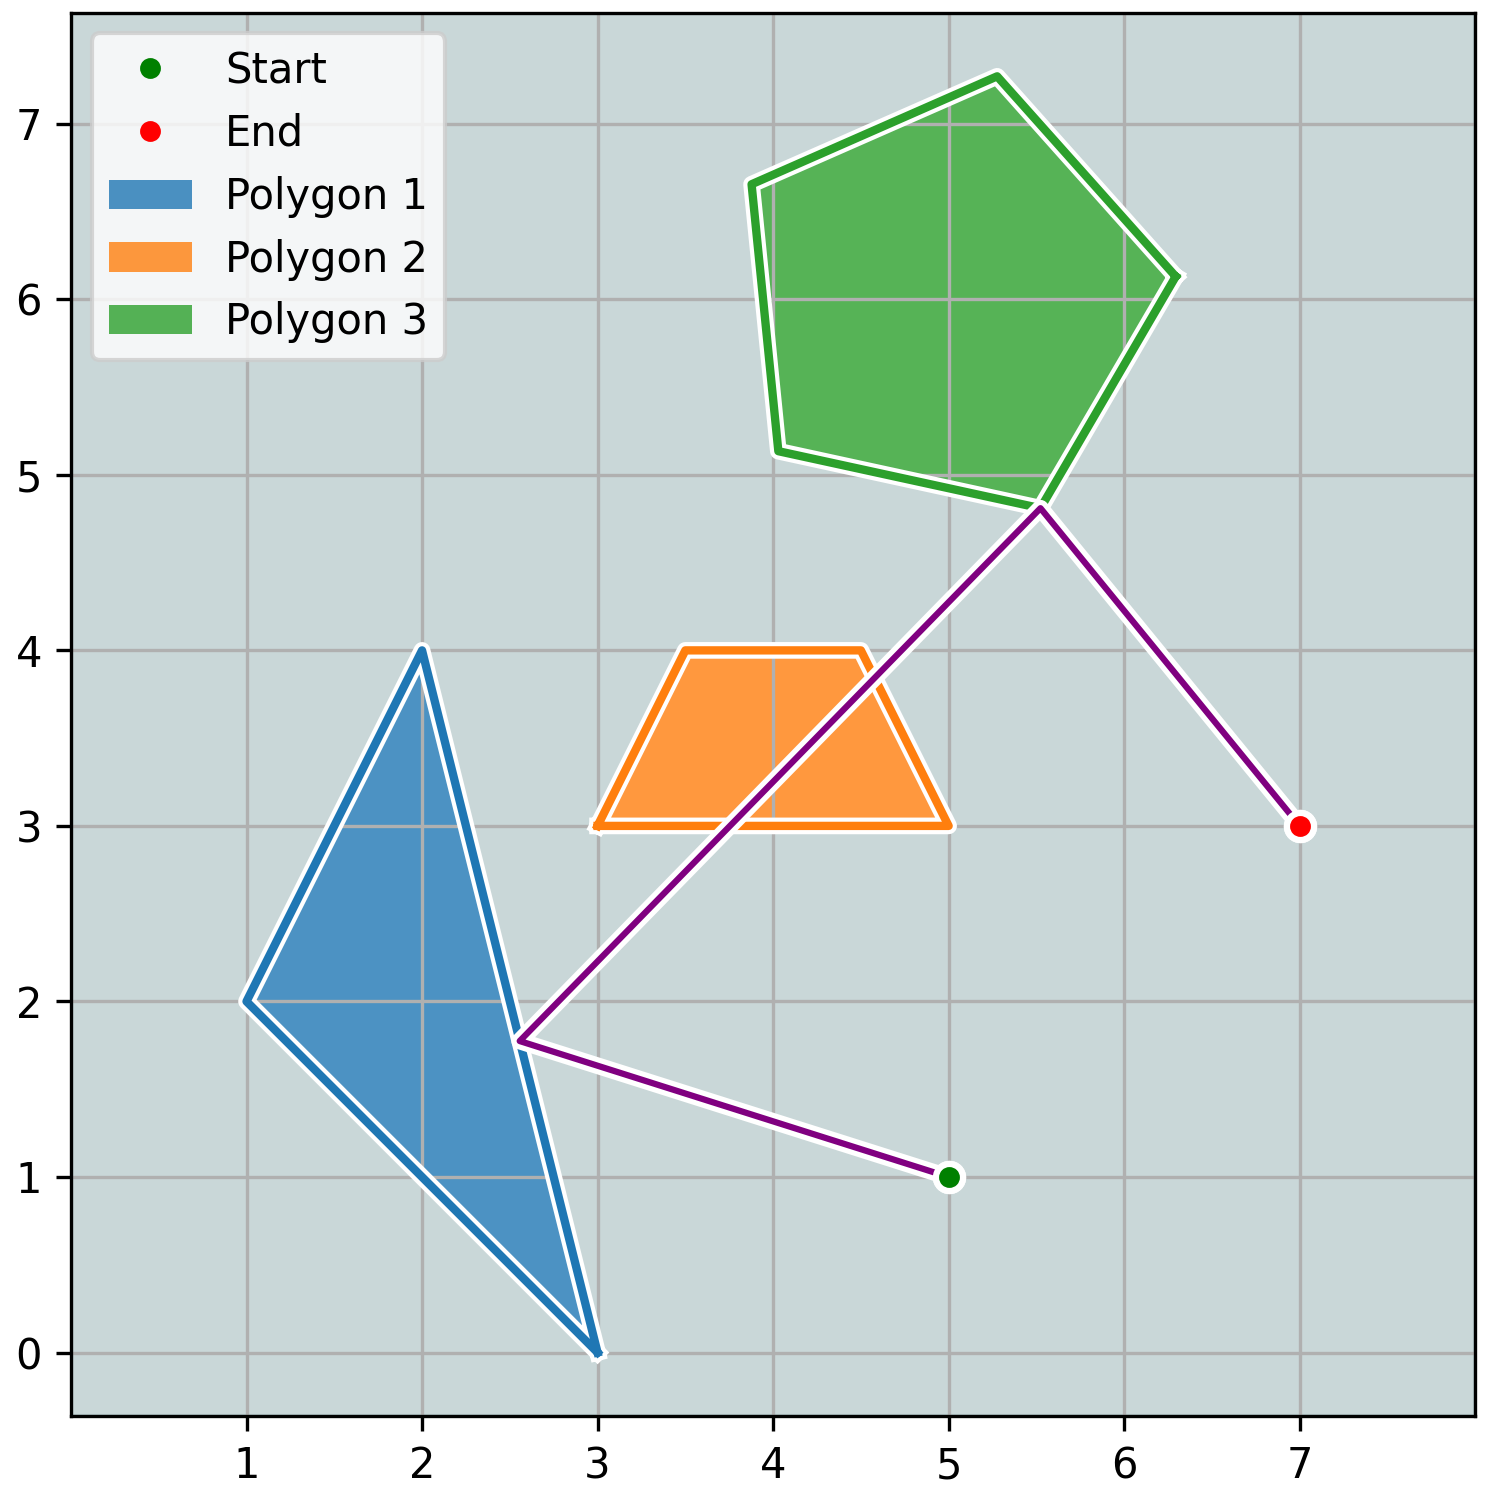
\includegraphics[width=0.39\textwidth]{problem1-solution.png}
	\caption{Caminho mínimo para um caso de 3 polígonos.}
\end{wrapfigure}

Considere o seguinte problema: dados dois pontos \(s, t \in \mathbb{R}^2\) e uma sequência de polígonos convexos disjuntos \(P_1, P_2, \ldots, P_k\), encontrar o caminho de menor comprimento que se inicia em \(s\), termina em \(t\) e toca cada polígono \(P_i\) em pelo menos um ponto, podendo atravessá-los.

A figura ao lado ilustra um exemplo de entrada e a solução ótima para o problema para um caso com 3 polígonos. Temos \(s\) 
como o \textcolor[RGB]{0,128,0}{ponto verde}, \(t\) como o \textcolor[RGB]{255, 0, 0}{ponto vermelho} e os polígonos \(P_1, P_2\) e \(P_3\) como o \textcolor[RGB]{76, 146, 195}{triângulo azul}, o \textcolor[RGB]{255, 152, 62}{trapézio laranja} e o \textcolor[RGB]{86, 179, 86}{pentágono verde}, respectivamente. O caminho mínimo é representado pela \textcolor[RGB]{145, 41, 145}{linha roxa}.
% como o ponto verde, \(t\) como o ponto vermelho e os polígonos \(P_1, P_2\) e \(P_3\) como o triângulo azul, o trapézio laranja e o pentágono verde, respectivamente. O caminho mínimo é representado pela linha roxa.

Retomando o paper, definimos um \(i\)-path até \(p\) como um caminho mínimo que começa em \(s\), encosta em cada um dos polígonos \(P_1, P_2, \ldots, P_i\) e termina em \(p\). Note que nosso objetivo é encontrar um \(k\)-path até \(t\). Enquanto não vamos entrar em detalhes, todo \(i\)-path é único.

A função central desse algoritmo será a função \(\text{Query}(p, i)\), que recebe um ponto \(p\) e um índice \(i\) e retorna o penúltimo ponto \(q\) do \(i\)-path até \(p\) (ou seja, o ponto imediatamente anterior a \(p\) nesse caminho). Note que a resposta do problema pode ser obtida chamando \(\text{Query}(t, k)\).

Primeiramente, vamos descrever procedimentos auxiliares que serão úteis para a implementação da função \(\text{Query}\). Finalmente, vamos descrever como respoder consultas usando esses procedimentos. Por enquanto, vamos assumir que sabemos como respoder as consultas.

\subsection{Particionando o Plano}

O primeiro passo do algoritmo é, para cada polígono \(P_i\), criar uma partição \(S_i\) do plano. Essa partição tem 3 tipos de regiões, 
% \textcolor[RGB]{255, 140, 140}{Regiões de Vértice}, \textcolor[RGB]{140, 197, 140}{Regiões de Aresta} e \textcolor[RGB]{150, 208, 209}{Regiões de Atravessa}.
\textcolor[RGB]{255, 70, 70}{Regiões de Vértice}, \textcolor[RGB]{86, 179, 86}{Regiões de Aresta} e \textcolor[RGB]{76, 146, 195}{Regiões de Atravessa}.
Essa partição é usada para responder consultas, uma vez que o comportamento da função \(\text{Query}(p, i)\) depende de qual região \(p\) pertence.

\subsubsection{Representado as Partições}

Primeiramente, note que as regiões de vértice são todas diversos `cones' associados à vértices do polígono \(P_i\), mais formalmente, cada região de vértices é a região do plano delimitada por duas semi-retas que partem de um vértice \(v\) de \(P_i\). Por esse motivo, pensamos em cada região de vértice como uma tripla \((v, d_1, d_2)\) respresentando o vértice, a direção da primeira semi-reta e a direção da segunda semi-reta. Também é importante ressaltar que a ordem das retas importa, assim consideramos que a região é o conjunto atingido por um movimento anti-horário a partir de \(d_1\) até \(d_2\).

A seguir, as regiões de aresta são todas diversas `faixas' associadas às arestas do polígono \(P_i\), mais formalmente, cada região de aresta é a região do plano delimitada por duas semi-retas que partem dos extremos de uma aresta \(e\) de \(P_i\) e a prórpia aresta \(e\). Por esse motivo, pensamos em cada região de aresta como uma quádrupla \((u, v, d_1, d_2)\) respresentando os dois extremos \(u\) e \(v\) da aresta, a direção da primeira semi-reta e a direção da segunda semi-reta. Aqui a ordem também importa, assim consideramos que a região é o conjunto atingido por um movimento anti-horário a partir de \(u\) e \(d_1\) até \(v\) e \(d_2\).

Finalmente, podemos dizer que as regiões de atravessa são todas as outras regiões do plano, ou seja, o complemento das regiões de vértice e aresta. Note que há exatamente uma região de atravessa.

\subsubsection{Construindo as Partições}

\begin{wrapfigure}{r}{0.60\textwidth}

\vspace{-15pt}
\centering
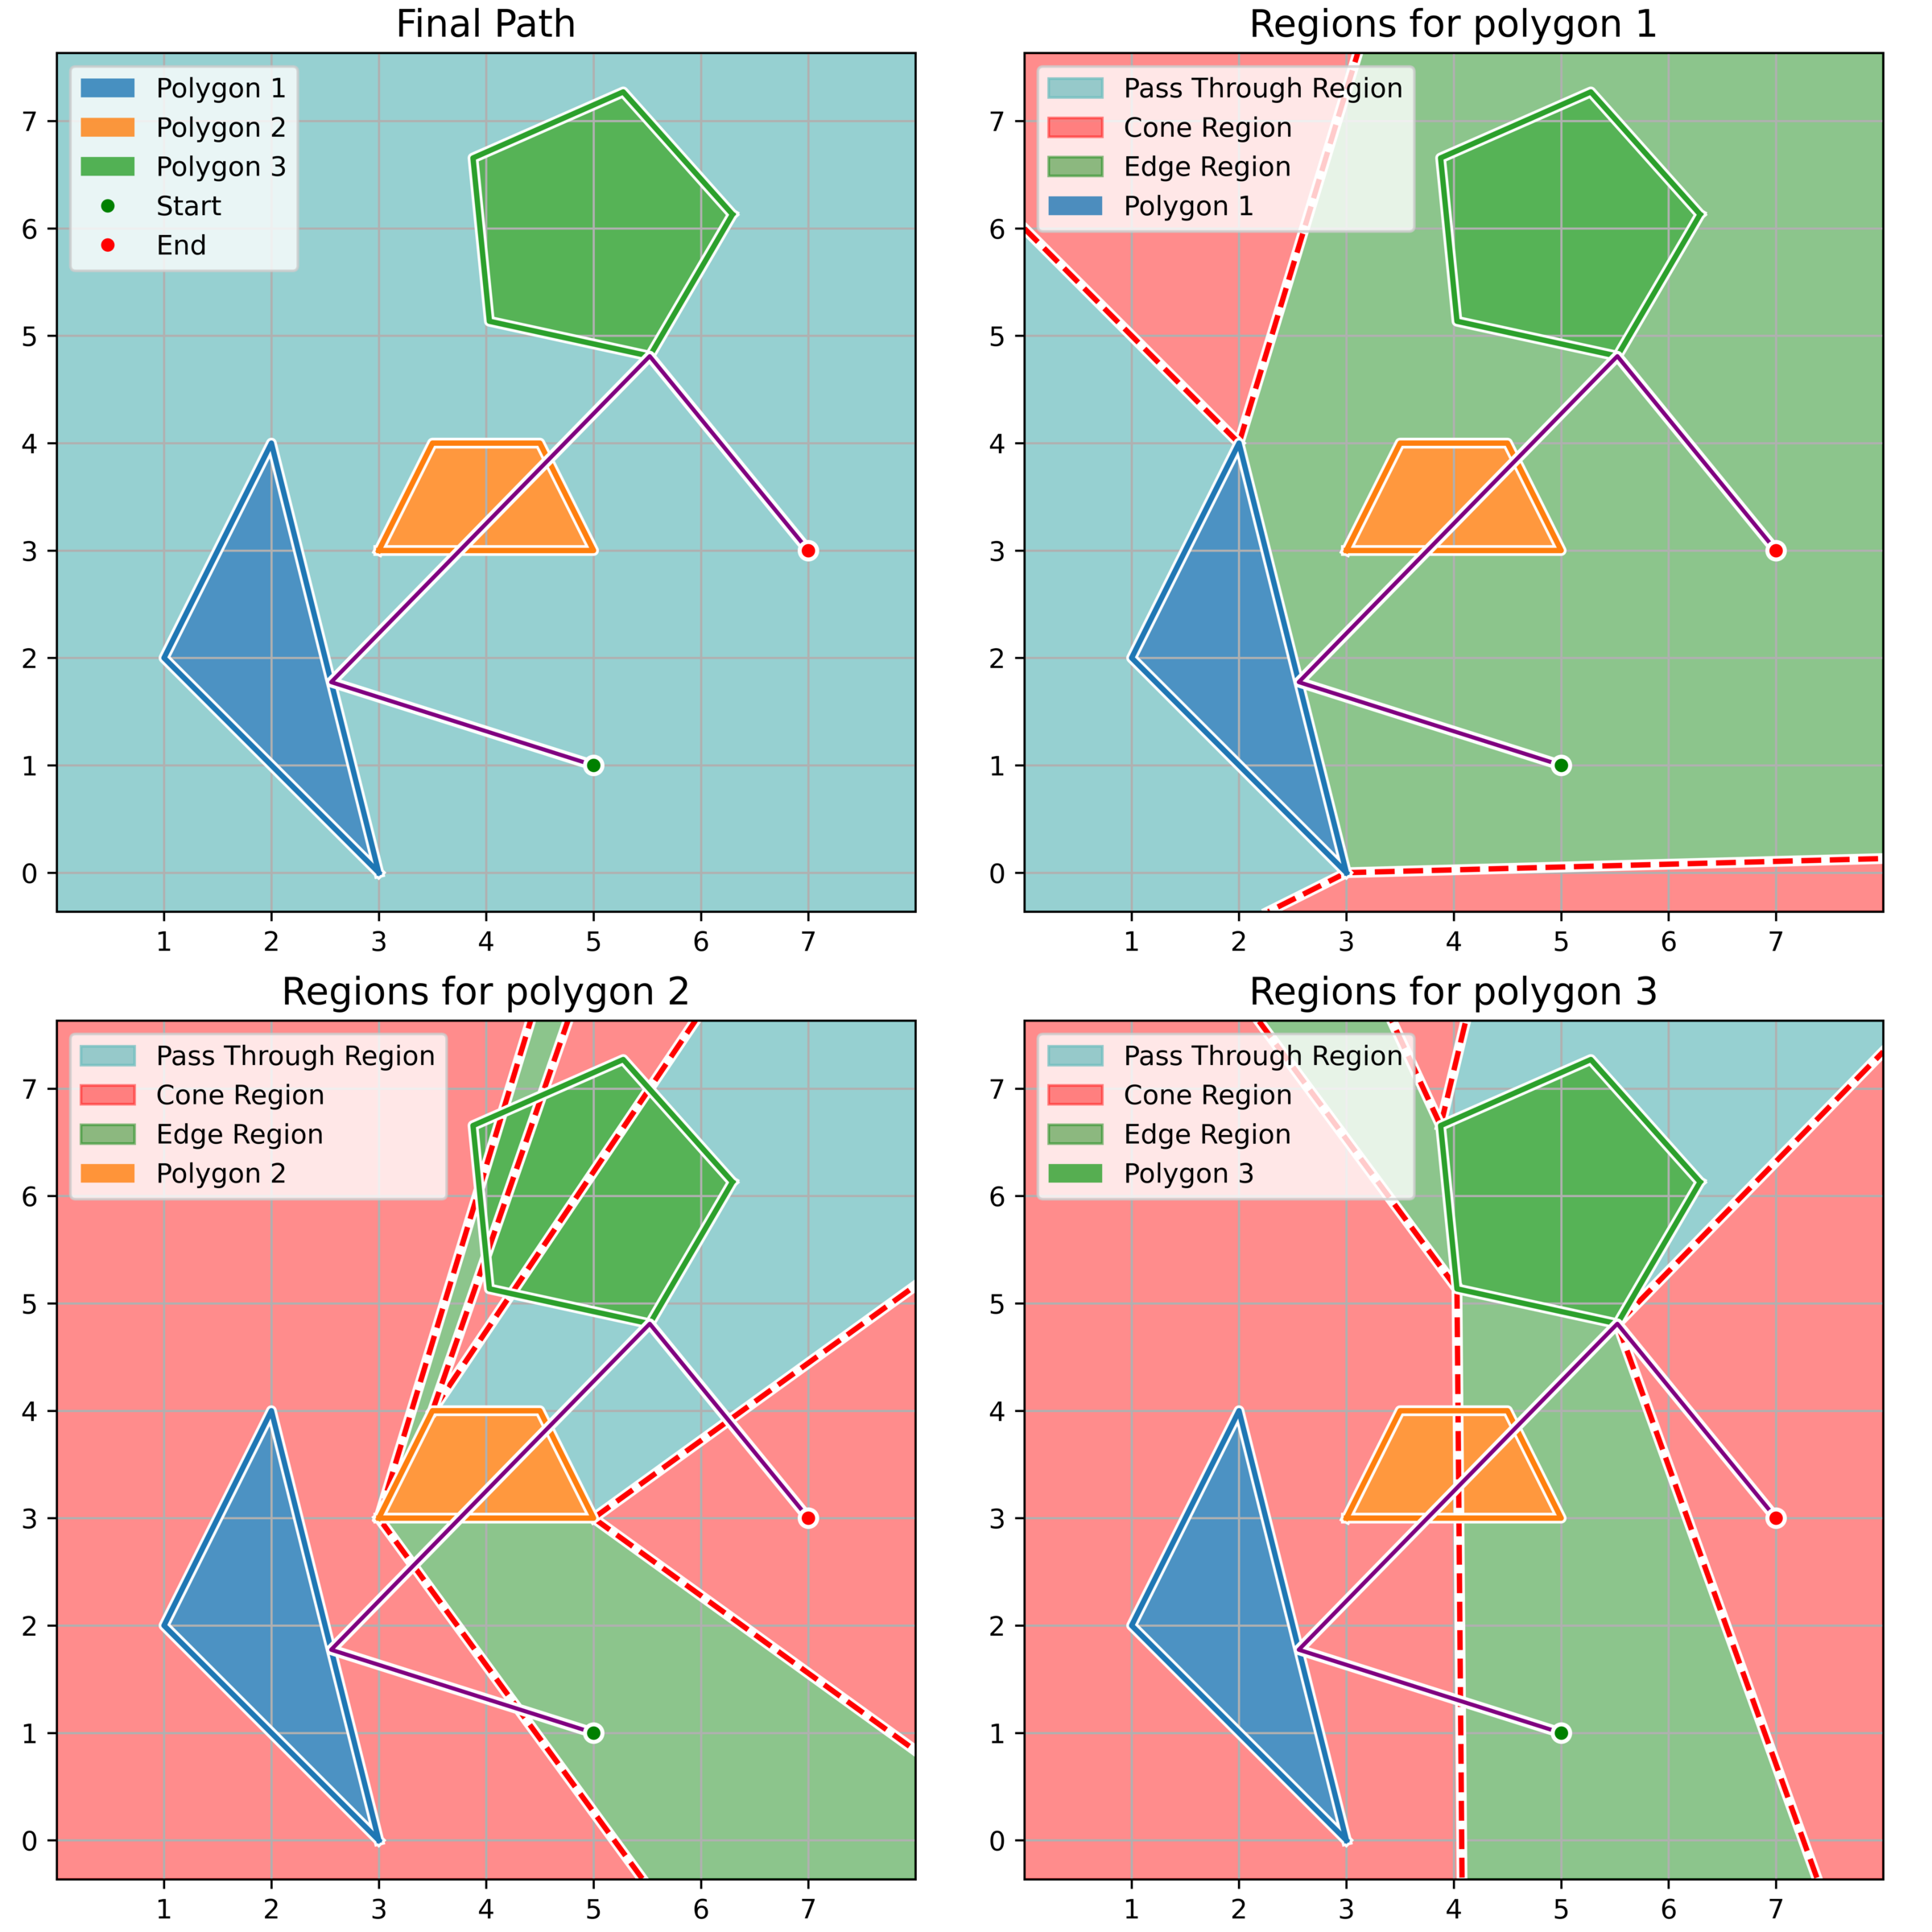
\includegraphics[width=0.6\textwidth]{problem1-partitions-reduced.png}
\caption{Partição do plano para cada poígono do exemplo anterior.}

\end{wrapfigure}

Primeiramente, a partir da figura, note que nem todo vértice e nem toda aresta de \(P_i\) geram uma região na partição \(S_i\). Dizemos que uma aresta que gera uma região é uma aresta visível, assim, nosso primeiro passo é encontrar todas as arestas visíveis de \(P_i\). 

Para deteminar se uma aresta \(e\) é visível, simplesmente calculamos \(p = \text{Query}(m, i)\) onde \(m\) é o ponto médio de \(e\) e verificamos se \(\overline{pm}\) atravessa \(P_i\). Se o segmento atravessa \(P_i\), então \(e\) não é visível, caso contrário, \(e\) é visível.

Uma vez que temos todas as arestas visíveis, podemos construir as regiões de vértice e de aresta. Para cada vértice \(v\) de \(P_i\), calculamos \(p = \text{Query}(v, i)\) e consideramos a direção de \(d = v - p\).
Se a aresta anterior a \(v\) (no sentido anti-horário) é visível, então \(d_1\) será a reflexão de \(d\) em relação à aresta anterior, caso contrário, \(d_1\) será a mesma direção de \(d\). Similarmente, se a aresta posterior a \(v\) é visível, então \(d_2\) será a reflexão de \(d\) em relação à aresta posterior, caso contrário, \(d_2\) será a mesma direção de \(d\). Assim, criamos a região de vértice \((v, d_1, d_2)\).

Dessa forma, sabemos todas as regiões de vértice. Agora para cada aresta visível \(e = (u, v)\) de \(P_i\), temos que \(d_1\) será a segunda direção da região de vértice associada a \(u\) e \(d_2\) será a primeira direção da região de vértice associada a \(v\). Assim, criamos a região de aresta \((u, v, d_1, d_2)\).

Finalmente, não é necessário criar a região de atravessa, uma vez que sabemos que um ponto pertence a ela se ele não pertence a nenhuma outra região.

\subsection{Respondendo Consultas}

Agora que sabemos como construir as partições \(S_i\), podemos descrever como usá-las para responder consultas \(\text{Query}(p, i)\). O procedimento utilizado é recursivo, assim, primeiro definimos o caso base, que é \(\text{Query}(p, 0) = s\), uma vez que um \(0\)-path não precisa tocar em nenhum polígono, assim, o menor caminho é uma linha reta de \(s\) até \(p\).

Para \(i > 0\), primeiramente determinamos a região \(R\) de \(S_i\) que contém \(p\). Descrevemos acima como representar cada região e a partir dela é fácil determinar à qual um ponto \(p\) pertence. Também é importante ressaltar que \(p\) sempre pertence a exatamente uma região. Agora vamos analisar os 3 casos possíveis para \(R\):

\begin{itemize}

	\item Região de Vértice: Seja \(R = (v, d_1, d_2)\). Nesse caso, o \(i\)-path até \(p\) é deve passar pelo vértice \(v\), tocando o polígono \(P_i\). Assim, temos que \(\text{Query}(p, i) = v\).
	
	\item Região de Aresta: Seja \(R = (u, v, d_1, d_2)\). Nesse caso, o \(i\)-path até \(p\) deve passar por algum ponto \(q\) da aresta \(e = (u, v)\), tocando o polígono \(P_i\). Para calcular \(q\), primeiro determinamos \(q' = \text{Query}(p', i - 1)\), onde \(p'\) é a reflexão de \(p\) em relação à aresta \(e\). 
	Agora, dizemos que \(q\) é a interseção entre \(\overline{q'p'}\) e a aresta \(e\). Finalmente, respondemos \(\text{Query}(p, i) = q\).

	\item Região de Atravessa: Seja \(R\) a região de atravessa. Nesse caso, o \(i\)-path até \(p\) automaticamente atravessa o polígono \(P_i\) em algum ponto. Portanto, podemos simplesmente responder \(\text{Query}(p, i) = \text{Query}(p, i - 1)\).

\end{itemize}

\subsection{Calculando o Caminho Mínimo}

Uma vez que sabemos como responder consultas, calcular o caminho final é muito simples. Basta calcular \(q_k = \text{Query}(t, k)\), então \(q_{k - 1} =\text{Query}(q_k, k - 1)\) e assim por diante, até \(q_0 = s\). Assim, o caminho mínimo é simplesmente a sequência \(s, q_1, \ldots, q_k, t\).

\section{O Problema de Visita de Polígonos Geral}

Vamos tomar como base a implementação do algoritmo de Mitchell para o problema restrito que fizemos em \textit{Python}. O código pode ser encontrado no arquivo \texttt{TouringPolygons/problem2.py}.

\subsection{Definições e Notação}

O problema segue de forma similar ao anterior, mas agora também recebemos como entrada `cercas' \(F_0, \dots, F_k\) tais que para todo \(0 \le i \le k\) vale que o polígono \(P_i\) e \(P_{i + 1}\) estão contidos em \(F_i\), para tal, consideramos \(P_0 = \{s\}\) e \(P_{k + 1} = \{t\}\). Nosso objetivo é encontrar o caminho de menor comprimento que se inicia em \(s\), termina em \(t\), toca cada polígono \(P_i\) em pelo menos um ponto e nunca sai da cerca \(F_i\) no seu caminho entre \(P_i\) e \(P_{i + 1}\).

\bibliography{referencias}

\end{document}
